\documentclass{article}
\usepackage[utf8]{inputenc}
\usepackage{tikz}
\usetikzlibrary{positioning,shapes.geometric}
\tikzstyle{carre}=[rectangle,rounded corners,draw=red!80,fill=red!10,inner ysep=0.2cm,text width=2cm,text centered]
\tikzstyle{losange}=[diamond,draw=blue!80,fill=blue!10, inner ysep=0.1cm,text width=1cm,text centered]
\tikzstyle{cercle}=[draw,circle]
\begin{document}

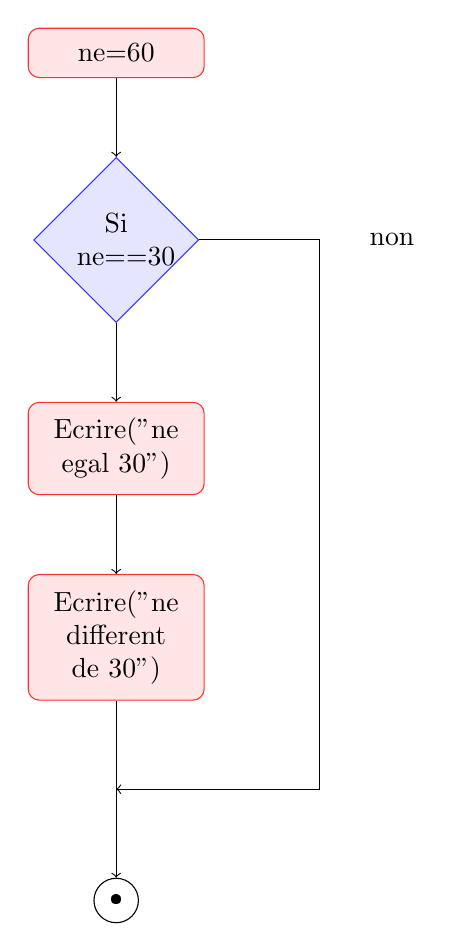
\begin{tikzpicture}

\node[carre] (A00)  {ne=60};
\node[losange] (S10) [below =of A00] {Si ne$=$=30};
\node (auxS10) [right = 4em of S10]{};
\node[carre] (E20) [below =of S10] {Ecrire("ne egal 30")};
\node[carre] (E30) [below =of E20] {Ecrire("ne different de 30")};
\node (FS40) [below =of E30] {};
\node[cercle] (C50) [below =of FS40] {\textbullet};

\draw [->](S10.east)|-(auxS10.center)node[pos=1.3,align=center]{non}|-(FS40.center);
\draw[->] (A00.south) to (S10.north);
\draw[->] (S10.south) to (E20.north);
\draw[->] (E20.south) to (E30.north);
\draw[->] (E30.south) to (C50.north);

\end{tikzpicture}

\end{document}
